\documentclass{standalone}
\usepackage{tikz}
\usetikzlibrary{patterns, positioning}


\begin{document}
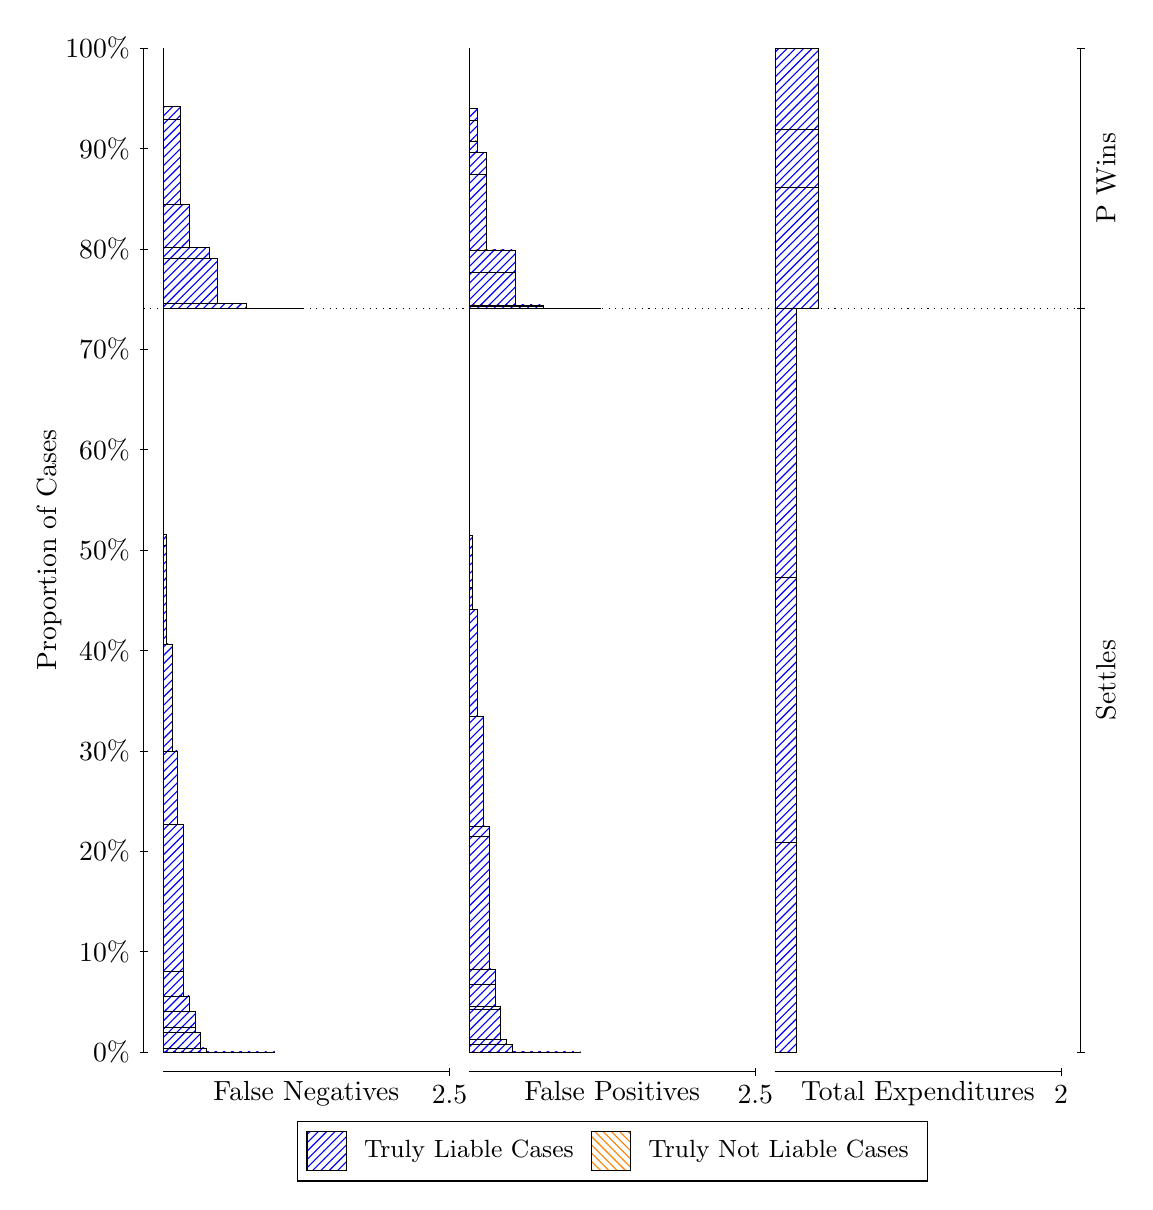
\begin{tikzpicture}
\draw[black, very thin] (1.5,1.75) -- (1.5,14.5);
\node[rotate=90, text=black, anchor=center] at (0.3, 8.125) {Proportion of Cases};
\draw[black, very thin] (1.45,1.75) -- (1.55,1.75);
\node[text=black, anchor=east] at (1.45, 1.75) {0\%};
\draw[black, very thin] (1.45,3.025) -- (1.55,3.025);
\node[text=black, anchor=east] at (1.45, 3.025) {10\%};
\draw[black, very thin] (1.45,4.3) -- (1.55,4.3);
\node[text=black, anchor=east] at (1.45, 4.3) {20\%};
\draw[black, very thin] (1.45,5.575) -- (1.55,5.575);
\node[text=black, anchor=east] at (1.45, 5.575) {30\%};
\draw[black, very thin] (1.45,6.85) -- (1.55,6.85);
\node[text=black, anchor=east] at (1.45, 6.85) {40\%};
\draw[black, very thin] (1.45,8.125) -- (1.55,8.125);
\node[text=black, anchor=east] at (1.45, 8.125) {50\%};
\draw[black, very thin] (1.45,9.4) -- (1.55,9.4);
\node[text=black, anchor=east] at (1.45, 9.4) {60\%};
\draw[black, very thin] (1.45,10.675) -- (1.55,10.675);
\node[text=black, anchor=east] at (1.45, 10.675) {70\%};
\draw[black, very thin] (1.45,11.95) -- (1.55,11.95);
\node[text=black, anchor=east] at (1.45, 11.95) {80\%};
\draw[black, very thin] (1.45,13.225) -- (1.55,13.225);
\node[text=black, anchor=east] at (1.45, 13.225) {90\%};
\draw[black, very thin] (1.45,14.5) -- (1.55,14.5);
\node[text=black, anchor=east] at (1.45, 14.5) {100\%};

\draw[black, very thin] (13.4,1.75) -- (13.4,14.5);
\draw[black, very thin] (13.35,1.75) -- (13.45,1.75);
\node[anchor=west] at (13.35, 1.75) {};
\draw[black, very thin] (13.35,11.197) -- (13.45,11.197);
\node[anchor=west] at (13.35, 11.197) {};
\draw[black, very thin] (13.35,14.5) -- (13.45,14.5);
\node[anchor=west] at (13.35, 14.5) {};

\draw[black, very thin, pattern color=blue, pattern=north east lines] (1.75,1.75) rectangle (3.167,1.75);
\draw[black, very thin, pattern color=blue, pattern=north east lines] (1.75,1.75) rectangle (3.0217,1.75);
\draw[black, very thin, pattern color=blue, pattern=north east lines] (1.75,1.75) rectangle (2.8763,1.75);
\draw[black, very thin, pattern color=blue, pattern=north east lines] (1.75,1.75) rectangle (2.8037,1.75);
\draw[black, very thin, pattern color=blue, pattern=north east lines] (1.75,1.75) rectangle (2.731,1.75);
\draw[black, very thin, pattern color=blue, pattern=north east lines] (1.75,1.75) rectangle (2.6583,1.75);
\draw[black, very thin, pattern color=blue, pattern=north east lines] (1.75,1.75) rectangle (2.5857,1.7504);
\draw[black, very thin, pattern color=blue, pattern=north east lines] (1.75,1.7504) rectangle (2.513,1.7504);
\draw[black, very thin, pattern color=blue, pattern=north east lines] (1.75,1.7504) rectangle (2.4403,1.7508);
\draw[black, very thin, pattern color=blue, pattern=north east lines] (1.75,1.7508) rectangle (2.3677,1.7508);
\draw[black, very thin, pattern color=blue, pattern=north east lines] (1.75,1.7508) rectangle (2.3677,1.7525);
\draw[black, very thin, pattern color=blue, pattern=north east lines] (1.75,1.7525) rectangle (2.295,1.8009);
\draw[black, very thin, pattern color=blue, pattern=north east lines] (1.75,1.8009) rectangle (2.2223,2.0027);
\draw[black, very thin, pattern color=blue, pattern=north east lines] (1.75,2.0027) rectangle (2.1497,2.0684);
\draw[black, very thin, pattern color=blue, pattern=north east lines] (1.75,2.0684) rectangle (2.1497,2.2618);
\draw[black, very thin, pattern color=blue, pattern=north east lines] (1.75,2.2618) rectangle (2.077,2.4629);
\draw[black, very thin, pattern color=blue, pattern=north east lines] (1.75,2.4629) rectangle (2.0043,2.4632);
\draw[black, very thin, pattern color=blue, pattern=north east lines] (1.75,2.4632) rectangle (2.0043,2.7686);
\draw[black, very thin, pattern color=blue, pattern=north east lines] (1.75,2.7686) rectangle (2.0043,4.6409);
\draw[black, very thin, pattern color=blue, pattern=north east lines] (1.75,4.6409) rectangle (1.9317,5.5747);
\draw[black, very thin, pattern color=blue, pattern=north east lines] (1.75,5.5747) rectangle (1.859,6.9316);
\draw[black, very thin, pattern color=blue, pattern=north east lines] (1.75,6.9316) rectangle (1.7863,8.1869);
\draw[black, very thin, pattern color=blue, pattern=north east lines] (1.75,8.1869) rectangle (1.7863,8.3242);
\draw[black, very thin, pattern color=orange, pattern=north west lines] (1.75,8.3242) rectangle (1.75,8.3242);
\draw[black, very thin, pattern color=blue, pattern=north east lines] (1.75,8.3242) rectangle (1.75,11.197);
\draw[black, very thin, pattern color=blue, pattern=north east lines] (1.75,11.197) rectangle (3.5303,11.197);
\draw[black, very thin, pattern color=blue, pattern=north east lines] (1.75,11.197) rectangle (3.167,11.198);
\draw[black, very thin, pattern color=blue, pattern=north east lines] (1.75,11.198) rectangle (3.058,11.198);
\draw[black, very thin, pattern color=blue, pattern=north east lines] (1.75,11.198) rectangle (2.8037,11.253);
\draw[black, very thin, pattern color=blue, pattern=north east lines] (1.75,11.253) rectangle (2.6947,11.253);
\draw[black, very thin, pattern color=blue, pattern=north east lines] (1.75,11.253) rectangle (2.4403,11.83);
\draw[black, very thin, pattern color=blue, pattern=north east lines] (1.75,11.83) rectangle (2.3313,11.965);
\draw[black, very thin, pattern color=blue, pattern=north east lines] (1.75,11.965) rectangle (2.077,12.518);
\draw[black, very thin, pattern color=blue, pattern=north east lines] (1.75,12.518) rectangle (1.968,13.589);
\draw[black, very thin, pattern color=blue, pattern=north east lines] (1.75,13.589) rectangle (1.968,13.76);
\draw[black, very thin, pattern color=orange, pattern=north west lines] (1.75,13.76) rectangle (1.75,13.76);
\draw[black, very thin, pattern color=blue, pattern=north east lines] (1.75,13.76) rectangle (1.75,14.5);
\draw[black, very thin, pattern color=orange, pattern=north west lines] (5.6333,1.75) rectangle (7.0503,1.75);
\draw[black, very thin, pattern color=blue, pattern=north east lines] (5.6333,1.75) rectangle (7.0503,1.75);
\draw[black, very thin, pattern color=orange, pattern=north west lines] (5.6333,1.75) rectangle (6.905,1.75);
\draw[black, very thin, pattern color=blue, pattern=north east lines] (5.6333,1.75) rectangle (6.905,1.75);
\draw[black, very thin, pattern color=orange, pattern=north west lines] (5.6333,1.75) rectangle (6.7597,1.75);
\draw[black, very thin, pattern color=blue, pattern=north east lines] (5.6333,1.75) rectangle (6.7597,1.75);
\draw[black, very thin, pattern color=blue, pattern=north east lines] (5.6333,1.75) rectangle (6.687,1.75);
\draw[black, very thin, pattern color=orange, pattern=north west lines] (5.6333,1.75) rectangle (6.6143,1.75);
\draw[black, very thin, pattern color=blue, pattern=north east lines] (5.6333,1.75) rectangle (6.6143,1.75);
\draw[black, very thin, pattern color=blue, pattern=north east lines] (5.6333,1.75) rectangle (6.5417,1.75);
\draw[black, very thin, pattern color=orange, pattern=north west lines] (5.6333,1.75) rectangle (6.469,1.75);
\draw[black, very thin, pattern color=blue, pattern=north east lines] (5.6333,1.75) rectangle (6.469,1.75);
\draw[black, very thin, pattern color=blue, pattern=north east lines] (5.6333,1.75) rectangle (6.3963,1.75);
\draw[black, very thin, pattern color=orange, pattern=north west lines] (5.6333,1.75) rectangle (6.3237,1.75);
\draw[black, very thin, pattern color=blue, pattern=north east lines] (5.6333,1.75) rectangle (6.3237,1.7508);
\draw[black, very thin, pattern color=orange, pattern=north west lines] (5.6333,1.7508) rectangle (6.3237,1.7508);
\draw[black, very thin, pattern color=blue, pattern=north east lines] (5.6333,1.7508) rectangle (6.3237,1.751);
\draw[black, very thin, pattern color=blue, pattern=north east lines] (5.6333,1.751) rectangle (6.251,1.7513);
\draw[black, very thin, pattern color=orange, pattern=north west lines] (5.6333,1.7513) rectangle (6.1783,1.7513);
\draw[black, very thin, pattern color=blue, pattern=north east lines] (5.6333,1.7513) rectangle (6.1783,1.8441);
\draw[black, very thin, pattern color=blue, pattern=north east lines] (5.6333,1.8441) rectangle (6.1057,1.9088);
\draw[black, very thin, pattern color=orange, pattern=north west lines] (5.6333,1.9088) rectangle (6.033,1.9088);
\draw[black, very thin, pattern color=blue, pattern=north east lines] (5.6333,1.9088) rectangle (6.033,2.2956);
\draw[black, very thin, pattern color=blue, pattern=north east lines] (5.6333,2.2956) rectangle (6.033,2.3295);
\draw[black, very thin, pattern color=blue, pattern=north east lines] (5.6333,2.3295) rectangle (5.9603,2.6053);
\draw[black, very thin, pattern color=blue, pattern=north east lines] (5.6333,2.6053) rectangle (5.9603,2.8061);
\draw[black, very thin, pattern color=orange, pattern=north west lines] (5.6333,2.8061) rectangle (5.8877,2.8061);
\draw[black, very thin, pattern color=blue, pattern=north east lines] (5.6333,2.8061) rectangle (5.8877,4.4851);
\draw[black, very thin, pattern color=blue, pattern=north east lines] (5.6333,4.4851) rectangle (5.8877,4.6226);
\draw[black, very thin, pattern color=blue, pattern=north east lines] (5.6333,4.6226) rectangle (5.815,6.0151);
\draw[black, very thin, pattern color=blue, pattern=north east lines] (5.6333,6.0151) rectangle (5.7423,7.3721);
\draw[black, very thin, pattern color=blue, pattern=north east lines] (5.6333,7.3721) rectangle (5.6697,7.6466);
\draw[black, very thin, pattern color=blue, pattern=north east lines] (5.6333,7.6466) rectangle (5.6697,8.3058);
\draw[black, very thin, pattern color=blue, pattern=north east lines] (5.6333,8.3058) rectangle (5.6333,11.197);
\draw[black, very thin, pattern color=orange, pattern=north west lines] (5.6333,11.197) rectangle (7.3047,11.197);
\draw[black, very thin, pattern color=blue, pattern=north east lines] (5.6333,11.197) rectangle (7.3047,11.197);
\draw[black, very thin, pattern color=orange, pattern=north west lines] (5.6333,11.197) rectangle (6.9413,11.197);
\draw[black, very thin, pattern color=blue, pattern=north east lines] (5.6333,11.197) rectangle (6.9413,11.197);
\draw[black, very thin, pattern color=blue, pattern=north east lines] (5.6333,11.197) rectangle (6.9413,11.197);
\draw[black, very thin, pattern color=orange, pattern=north west lines] (5.6333,11.197) rectangle (6.578,11.197);
\draw[black, very thin, pattern color=blue, pattern=north east lines] (5.6333,11.197) rectangle (6.578,11.223);
\draw[black, very thin, pattern color=blue, pattern=north east lines] (5.6333,11.223) rectangle (6.578,11.237);
\draw[black, very thin, pattern color=orange, pattern=north west lines] (5.6333,11.237) rectangle (6.469,11.237);
\draw[black, very thin, pattern color=blue, pattern=north east lines] (5.6333,11.237) rectangle (6.469,11.237);
\draw[black, very thin, pattern color=orange, pattern=north west lines] (5.6333,11.237) rectangle (6.2147,11.237);
\draw[black, very thin, pattern color=blue, pattern=north east lines] (5.6333,11.237) rectangle (6.2147,11.651);
\draw[black, very thin, pattern color=blue, pattern=north east lines] (5.6333,11.651) rectangle (6.2147,11.936);
\draw[black, very thin, pattern color=orange, pattern=north west lines] (5.6333,11.936) rectangle (6.1057,11.936);
\draw[black, very thin, pattern color=blue, pattern=north east lines] (5.6333,11.936) rectangle (6.1057,11.936);
\draw[black, very thin, pattern color=blue, pattern=north east lines] (5.6333,11.936) rectangle (6.1057,11.937);
\draw[black, very thin, pattern color=blue, pattern=north east lines] (5.6333,11.937) rectangle (5.8513,12.891);
\draw[black, very thin, pattern color=blue, pattern=north east lines] (5.6333,12.891) rectangle (5.8513,13.179);
\draw[black, very thin, pattern color=blue, pattern=north east lines] (5.6333,13.179) rectangle (5.7423,13.32);
\draw[black, very thin, pattern color=orange, pattern=north west lines] (5.6333,13.32) rectangle (5.7423,13.32);
\draw[black, very thin, pattern color=blue, pattern=north east lines] (5.6333,13.32) rectangle (5.7423,13.579);
\draw[black, very thin, pattern color=blue, pattern=north east lines] (5.6333,13.579) rectangle (5.7423,13.731);
\draw[black, very thin, pattern color=blue, pattern=north east lines] (5.6333,13.731) rectangle (5.6333,14.5);
\draw[black, very thin, pattern color=orange, pattern=north west lines] (9.5167,1.75) rectangle (9.7892,1.75);
\draw[black, very thin, pattern color=blue, pattern=north east lines] (9.5167,1.75) rectangle (9.7892,4.4096);
\draw[black, very thin, pattern color=orange, pattern=north west lines] (9.5167,4.4096) rectangle (9.7892,4.4096);
\draw[black, very thin, pattern color=blue, pattern=north east lines] (9.5167,4.4096) rectangle (9.7892,7.7757);
\draw[black, very thin, pattern color=orange, pattern=north west lines] (9.5167,7.7757) rectangle (9.7892,7.7757);
\draw[black, very thin, pattern color=blue, pattern=north east lines] (9.5167,7.7757) rectangle (9.7892,11.197);
\draw[black, very thin, pattern color=orange, pattern=north west lines] (9.5167,11.197) rectangle (10.062,11.197);
\draw[black, very thin, pattern color=blue, pattern=north east lines] (9.5167,11.197) rectangle (10.062,12.726);
\draw[black, very thin, pattern color=orange, pattern=north west lines] (9.5167,12.726) rectangle (10.062,12.726);
\draw[black, very thin, pattern color=blue, pattern=north east lines] (9.5167,12.726) rectangle (10.062,13.462);
\draw[black, very thin, pattern color=orange, pattern=north west lines] (9.5167,13.462) rectangle (10.062,13.462);
\draw[black, very thin, pattern color=blue, pattern=north east lines] (9.5167,13.462) rectangle (10.062,14.5);
\draw[black, dotted] (1.5,11.197) -- (13.4,11.197);
\draw[black, very thin] (1.75,1.5) -- (5.3833,1.5);
\node[text=black, anchor=north] at (3.5667, 1.5) {False Negatives};
\draw[black, very thin] (5.3833,1.45) -- (5.3833,1.55);
\node[text=black, anchor=north] at (5.3833, 1.45) {2.5};

\draw[black, very thin] (5.6333,1.5) -- (9.2667,1.5);
\node[text=black, anchor=north] at (7.45, 1.5) {False Positives};
\draw[black, very thin] (9.2667,1.45) -- (9.2667,1.55);
\node[text=black, anchor=north] at (9.2667, 1.45) {2.5};

\draw[black, very thin] (9.5167,1.5) -- (13.15,1.5);
\node[text=black, anchor=north] at (11.333, 1.5) {Total Expenditures};
\draw[black, very thin] (13.15,1.45) -- (13.15,1.55);
\node[text=black, anchor=north] at (13.15, 1.45) {2};

\node[text=black, centered, rotate=90] at (13.72, 6.4734) {Settles};
\node[text=black, centered, rotate=90] at (13.72, 12.848) {P Wins};

\draw (7.449999999999999,1.5) node[draw=none] (baseCoordinate) {};
\begin{scope}[align=center]
        \matrix[scale=0.5, draw=black, below=0.5cm of baseCoordinate, nodes={draw}, column sep=0.1cm]{
            \node[rectangle, draw, minimum width=0.5cm, minimum height=0.5cm, pattern color=blue, pattern=north east lines] {}; &
            \node[draw=none, font=\small, text=black] (B) {Truly Liable Cases}; &
            \node[rectangle, draw, minimum width=0.5cm, minimum height=0.5cm, pattern color=orange, pattern=north west lines] {}; &
            \node[draw=none, font=\small, text=black] (B) {Truly Not Liable Cases}; \\
            };
\end{scope}

\end{tikzpicture}
\end{document}